\subsection{Gyroskop}
Et gyroskop er et elektromekanisk apparat, som anvendes til at måle vinkelændringer om en given akse, hvilket illustreres på \figref{fig:gyro}. Enhederne for data fra et gyroskop er grader per sekund (dps). Et gyropskop kan give information om orienteringen eller navigationen af objektet, som sensoren optager data fra. Hvis et gyroskop eksempelvis drejes én omgang om egen akse i sekundet, vil den registrere en vinkelændring på 360 dps. \citep{Sparkfun_gyro,Barbour2014} \newline
Et gyroskop kan eksempelvis registrere vinkelhastighed ved at anvende tyngdekræften og en lille indre masse \citep{Sparkfun_gyro,Barbour2014}.
\begin{figure}[H]
	\centering
	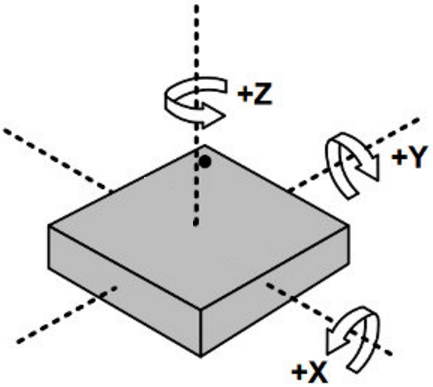
\includegraphics[scale=0.6]{figures/bProblemloesning/gyro.png}
	\caption{På figuren ses et gyroskops måling af rotation omkring x-, y- og z-aksen. \citep{Sparkfun_gyro} (Modificeret)}
	\label{fig:gyro}
\end{figure}\vspace{-.2cm}
Hvis et gyroskop eksempelvis opsamler data ved cykling, mens det er placeret på benet, vil massen blive udsat for en roterende bevægelse omkring den horisontale akse. Massen vil blive henholdsvis tungere og lettere i processen på baggrund af de ydre påvirkende kræfter, hvorfor outputtet vil komme til udtryk som en sinus-bølge. Outputtet er afhængig af tyngdekræftens påvirkning af massen, hvorfor et varierende output kræver en bevægelse. \citep{TittertonWeston2004,LuingeVeltink2005}
% Gyroskopet vil, uafhængigt af placering, have et fast output, som det vil vende tilbage til efter en bevægelse.
%Et gyroskop fungere ved at anvende inerti egenskaberne der opstår når et hjul spindes med en høj hastighed. Ved at hjulet fastholder den samme retning omkring aksen, kan impulsmomentmomentet, dets inertiprodukt samt hastighed være med til at definere en referenceretning. 
%De fundementale principper bag virkningen af et gyroskop er blandt andet det gyroskopiske inerti, som er når hjulet drejer om sin egen akse og står vinkelret på aksen. impulsmomentet som er fordelingen af en masse på et rotor, hvor vinkelhastigheden også har en betydning, og præcession som er rotationen omkring egen akse. 
%De signaler som opfanges af et accelerometrer, inkluderer ikke signaler fra den roterende akse og derfor kan en præcis orientering ikke opfanges. For at forbedre nøjagtigheden, kan man anvende gyroskoper som et supplement til accelerometre .
%Et gyroskop måler vinkelhastighed, hvor ændringen i orientering kan måles ved at integrere vinkelhastigheden på baggrund af en algoritme. \citep{LuingeVeltink2005}
%
\subsection{Vurdering af accelerometer og gyroskop i forhold til anvendelse}\label{acc_og_gyro}
Et accelerometer kan bestemme den g påvirkning, som et objekt udsættes for ved en given kraftpåvirkning, hvormed accelerometers ouput angives i $g$. Derimod bestemmer et gyroskop vinkelændringerne, som et objekt kan blive udsat for, hvoraf gyroskopers output angives i dps. Et gyroskop er, modsat et accelerometer, ikke markant påvirkeligt overfor støj og vibrationer. \citep{Goodrich2013,TittertonWeston2004,LuingeVeltink2005} \newline
Ydermere har et accelerometer og et gyroskop den væsentlige forskel, at et gyroskop har et større strømforbrug sammenlignet med et accelerometer. Et gyroskop er fordelagtig at benytte til blandt andet detektering af gang, løb og cykling. Gyroskopet har dog et så stort strømforbrug i forhold til et accelerometer, at den oftest udskiftes med et accelerometer til detektering af gang og løb. Dette fremgår yderligere af en række studier, som alle benytter accelerometer til detektering af gang og løb. \citep{Rueterbories2010,Sparkfun,ClelandKikhia2013} \newline
Som beskrevet i \secref{bevaegelse} er der en stor påvirkning af et accelerometer i y-aksens retning ved aktiviteterne gang og løb. Et accelerometer er derfor fordelagtigt at benytte til detektering af disse aktivitetsformer for at reducere strømforbruget. Dette er grundet sensorens lave strømforbrug, og et accelerometer kan bestemme de karakteristiske kraftpåvirkninger opstået ved gang og løb. Derimod er et gyroskop fordelagtigt at benytte til detektering af cykling, idet denne bevægelse er en cirkulær bevægelse omkring én akse. Betydningen heraf vil medføre, at cykling tilnærmelsesvis kan afspejles som en sinus bølge med varierende frekvens afhængigt af hastigheden. \citep{TittertonWeston2004,LuingeVeltink2005} \newline
I dette projekt vil der derfor blive benyttet et accelerometer til detektering af gang og løb og et gyroskop til detektering af cykling. Grundet strømforbruget af gyroskopet vil det være fordelagtigt, at denne sensor udelukkende er aktiv under og til detektering af cykling.% Denne store forskel i forbrug gør det også fordelagtigt, at gyroskopet kun skal tændes når der skal detekteres cykling.
